
\documentclass[11pt]{exam} % https://www.ctan.org/pkg/exam?lang=en

\usepackage[lmargin=1.in,rmargin=1.in,tmargin=1.in,bmargin=1in]{geometry}
\usepackage{setspace}
\usepackage[pdftex]{graphicx}
\usepackage{titling}
\usepackage[
	pdfauthor={Brian Weinstein},
	pdftitle={Homework 2},
	bookmarks=true,
	colorlinks=true,
	linkcolor=blue,
	urlcolor=blue,
	citecolor=blue,
	pdftex,
	linktocpage=true
	]{hyperref}
\usepackage[textsize=tiny]{todonotes}
\usepackage{float}
\setlength\parindent{0pt}


\qformat{\textbf{Question \thequestion: \thequestiontitle}\quad \hfill}


\pagestyle{headandfoot}
\runningheadrule
\firstpageheader{}{}{}
\runningheader{\thetitle}{\theauthor}{\thedate}
\firstpagefooter{}{}{}
\runningfooter{}{}{}

\usepackage{lipsum}


\begin{document}


\title{STAT S4240 002, Homework 2}
\author{Brian Weinstein (bmw2148)}
\date{July 23, 2015}
\maketitle



\begin{questions}



\titledquestion{\href{http://www-bcf.usc.edu/~gareth/ISL/}{James} 2.4, Exercise 8}

\lipsum[3]

\begin{parts}
	\part
	\lipsum[2]
	
	\part
	\lipsum[2]
\end{parts}

\titledquestion{\href{http://www-bcf.usc.edu/~gareth/ISL/}{James} 2.4, Exercise 8}

\lipsum[3]

\begin{parts}
	\part
	\lipsum[2]
	
	\part
	\lipsum[2]
\end{parts}


%\begin{figure}[H]
%	\centering
%	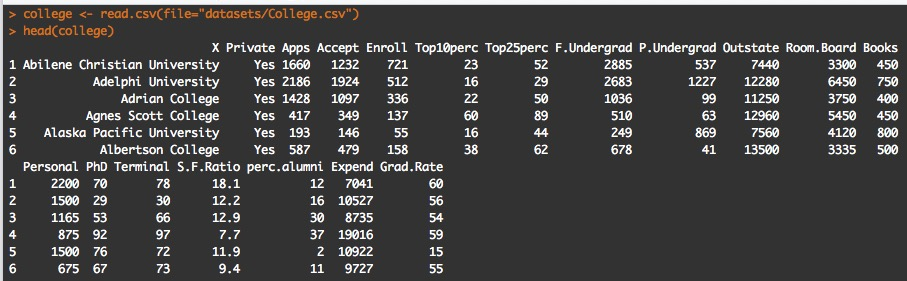
\includegraphics[width=6.5in]{8a.jpeg}
%	%\caption{}
%	%\label{fig:figName}
%\end{figure}


\end{questions}

\end{document}